\documentclass[a4paper,11pt]{article}

\usepackage{latexsym}
\usepackage{graphicx}
\usepackage{float}
\usepackage[margin=2cm]{geometry}
\usepackage{lscape}
\usepackage{underscore}
\usepackage{amsmath}
\usepackage{blindtext}
\usepackage{listings}
\usepackage{xcolor}
\usepackage{mathtools}

\usepackage[all]{nowidow}

\usepackage[LY1]{fontenc}
\usepackage[utf8x]{inputenc}
\usepackage{polski}
\usepackage[lf,enc=t1]{berenis}

\DeclareTextCompositeCommand{\k}{LY1}{a}
  {\oalign{a\crcr\noalign{\kern-.27ex}\hidewidth\char7}}


\usepackage{listings}
\usepackage{color}

\definecolor{mygreen}{rgb}{0,0.6,0}
\definecolor{mygray}{rgb}{0.5,0.5,0.5}
\definecolor{mymauve}{rgb}{0.58,0,0.82}

\lstset{ %
  backgroundcolor=\color{white},   % choose the background color; you must add \usepackage{color} or \usepackage{xcolor}; should come as last argument
  basicstyle=\footnotesize,        % the size of the fonts that are used for the code
  breakatwhitespace=false,         % sets if automatic breaks should only happen at whitespace
  breaklines=true,                 % sets automatic line breaking
  captionpos=b,                    % sets the caption-position to bottom
  commentstyle=\color{mygreen},    % comment style
  deletekeywords={...},            % if you want to delete keywords from the given language
  escapeinside={\%*}{*)},          % if you want to add LaTeX within your code
  extendedchars=true,              % lets you use non-ASCII characters; for 8-bits encodings only, does not work with UTF-8
  frame=single,	                   % adds a frame around the code
  keepspaces=true,                 % keeps spaces in text, useful for keeping indentation of code (possibly needs columns=flexible)
  keywordstyle=\color{blue},       % keyword style
  language=Java,                 % the language of the code
  morekeywords={*,...},            % if you want to add more keywords to the set
  numbers=left,                    % where to put the line-numbers; possible values are (none, left, right)
  numbersep=5pt,                   % how far the line-numbers are from the code
  numberstyle=\tiny\color{mygray}, % the style that is used for the line-numbers
  rulecolor=\color{black},         % if not set, the frame-color may be changed on line-breaks within not-black text (e.g. comments (green here))
  showspaces=false,                % show spaces everywhere adding particular underscores; it overrides 'showstringspaces'
  showstringspaces=false,          % underline spaces within strings only
  showtabs=false,                  % show tabs within strings adding particular underscores
  stepnumber=2,                    % the step between two line-numbers. If it's 1, each line will be numbered
  stringstyle=\color{mymauve},     % string literal style
  tabsize=2,	                   % sets default tabsize to 2 spaces
  title=\lstname                   % show the filename of files included with \lstinputlisting; also try caption instead of title
}



\begin{document}
\begin{titlepage}


\newcommand{\HRule}{\rule{\linewidth}{0.5mm}}
\center

\textsc{\LARGE Politechnika Wrocławska}\\[1.5cm]
\textsc{\LARGE Projektowanie efektywnych algorytmów}\\[0.5cm]

\HRule \\[0.5cm]
{ \huge \bfseries Projekt nr 2: \\[0.3cm]Implementacja i analiza efektywności algorytmu opartego na metodzie Tabu Search dla problemu komiwojażera }\\[0.5cm] 
\HRule \\[1.5cm]

\begin{flushleft} \large
 
\emph{Autor:}\\
 
Bartosz  \textsc{Pogoda} 225988 \\
 
\end{flushleft}
%\end{minipage}
 
%\begin{minipage}{0.4\textwidth}
\begin{flushright} \large
 
\emph{Prowadzący:} \\
dr inż. Jarosław \textsc{Mierzwa} 
 
\end{flushright}
%\end{minipage}\\[4cm]
 
\vfill
{\large 18 grudnia 2017}\\[3cm] 
 
 
\end{titlepage}

\tableofcontents
\newpage

\section{Wstęp teoretyczny}

\subsection{Opis algorytmu}

Problem komiwojażera definiowany jest dla grafów pełnych. Wierzchołki grafu nazywane są miastami,
a krawędziom przypisane są wartości reprezentujące odległości między nimi. Problem polega na
odnalezieniu najkrótszej ścieżki, takiej aby odwiedzić każde miasto dokładnie raz i wrócić do punktu
wyjścia. \newline
Wiele problemów, występujących w sektorach takich jak transport oraz logistyka można sprowadzić
do problemu komiwojażera. Zastosowanie efektywnych algorytmów rozwiązujących ten problem nie
rzadko prowadzi do redukcji kosztów i optymalizacji pewnych rzeczywistych procesów. Przykładową
aplikacją mogło by być wyznaczenie optymalnej trasy dla autobusu szkolnego, tak aby odwiedził
wszystkie przystanki z dziećmi w jak najkrótszym okresie czasu. Wierzchołkami grafu byłyby
poszczególne przystanki, a wartościami na krawędziach szacunkowy czas przemieszczenia się autobusu
między przystankami. Warto tutaj zauważyć, że czas przemieszczania się z przystanku A do B, może
różnić się od czasu przemieszczenia z B do A. Różnice te są uwzględnione w asymetrycznym problemie
komiwojażera, który zostanie poddany analizie w tym sprawozdaniu.

\subsection{Przeszukiwanie lokalne, sąsiedztwo}

Algorytm przeszukiwania lokalnego dla problemu komwijażera polega na poszukiwaniu lepszych rozwiązań zbliżonych do aktualnego rozwiązania. Dla rozwiązania definiuje się sąsiedztwo, czyli zbiór pobliskich rozwiązań. Pobliskich czyli takich, które można osiągnać poprzez wykonanie jednego ruchu na przykład może to być zamiana dwóch pozycji w aktualnej ścieżce (z wyłączeniem miasta startowego). Następnie z sąsiedztwa aktualnego rozwiązania wybiera się rozwiązanie najlepsze (najkrótsza ścieżka) i nastepuje kolejna iteracja algorytmu. Algorytm taki nie daje gwarancji znalezienia rozwiązania optymalnego, a nawet gdy takie znajdzie - nie mamy informacji o tym, że rozwiązanie to jest optymalne i możemy zakończyć poszukiwania. 

\subsection{Przeszukiwanie z zakazami}

Algorytm przeszkukiwania lokalnego ma poważną wadę, która znacznie ogranicza jego zastosowanie. Algorytm bardzo często osiąga minimum lokalne, z którego nie jest w stanie wyjść. Ten problem rozwiązuje zastosowanie metodyki Tabu Search - przeszukiwania z zakazami.

\subsubsection{Lista Tabu}

Lista Tabu zawiera ruchy, które zostały wykonane w niedalekiej przeszłości. Ruchy te są zakazane, dzięki czemu algorytm otrzymuje mechanikę pozwalającą na wydostanie się z minimum lokalnego, ponieważ do raz osiągniętego minimum nie będzie mógł wrócić przez jakiś czas. Ilość kroków, podczas których ruch jest zakazany określany jest jako kadencja. Parametr ten jest bardzo istotny, jego wybór znacząco wpływa na działanie algorytmu.
\subsubsection{Dywersyfikacja}

Dywersyfikacja jest kolejnym mechanizmem unikania minimum lokalnego. Polega ona na wybraniu rozwiązania potencjalnie odległego od aktualnego rozwiązania (np. rozwiązania losowego) w przypadku braku poprawy wyniku przez określony okres działania algorytmu.

\newpage
\section{Implementacja algorytmu, opis istotnych klas}
\subsection{Instancja}

Klasa reprezentująca instancję problemu. Przechowuje informacje o krawędziach w postaci macierzy sąsiedztwa. Została również utworzona funkcja pozwalająca na obliczenie długości podanej ścieżki w obrębie instancji - calculateTotalDistance.

\begin{figure}[H]
\centering
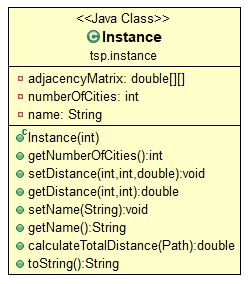
\includegraphics[height=7cm]{ClassInstance.JPG}
\caption{Deklaracja klasy Instance}
\end{figure}


\subsection{Instancja - odczyt z pliku}

Klasa usługowa tworząca instancje problemu (typ Instance) na podstawie plików w formatach TSPLIB95 (http://comopt.ifi.uni-heidelberg.de/software/TSPLIB95/). Klasa obudowuje bibliotekę jorlib, która została wykorzystana w celu odczytu wszystkich formatów plików pozyskanych z wyżej wymienionej strony. Wewnątrz metody read dosyć skomplikowany obiekt typu TSPLibInstance, otrzymany po przetworzeniu pliku przez bibliotekę jorlib, jest parsowany do obiektu typu Instance, zawierającego jedynie dane ważne z punktu widzenia projektu.

\begin{figure}[H]
\centering
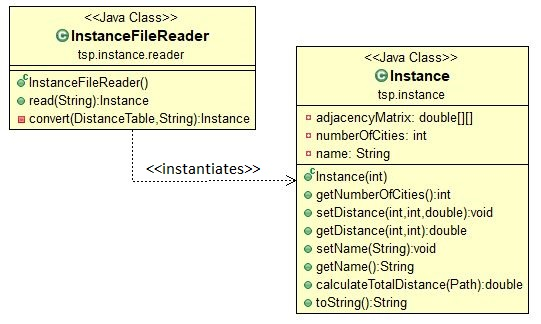
\includegraphics[height=8cm]{ClassInstanceFileReader.JPG}
\caption{Deklaracja klasy InstanceFileReader}
\end{figure}

\subsection{Ścieżka - rozwiązanie}

Klasa Path reprezentuje rozwiązanie algorytmu. Ścieżka jest w postaci [0, 1, 2, 3, 4, 0]. Pierwszy i ostatni element jest ustawiany za pomocą funkcji setStartCity, nie powinien on być zmieniany za pomocą funkcji setCity. Ścieżka posiada długość o jeden większą od rozmiaru instancji. 

\begin{figure}[H]
\centering
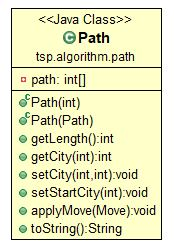
\includegraphics[height=8cm]{ClassPath.JPG}
\caption{Deklaracja klasy Path}
\end{figure}

\subsection{Ograniczenie czasowe algorytmu}

W celu umożliwienia zatrzymania algorytmu po zadanym czasie został zdefiniowany wątek AlgorithmTerminator.

\begin{figure}[H]
\centering
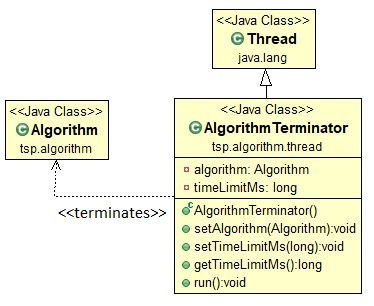
\includegraphics[height=8.5cm]{ClassAlgorithmTerminator.JPG}
\caption{Deklaracja klasy AlgorithmTerminator}
\end{figure}

\newpage
\subsection{Dywersyfikacja}

W ramach realizacji dywersyfikacji w projekcie został utworzony watek DiversificationChecker, który co ustalony czas sprawdza, czy wynik w aktualnym przedziale dywersyfikacji poprawił się (od czasu ostatniego sprawdzenia). W przypadku braku poprawy wyniku, wątek ustawia flagę dywersyfikacji na obiekcie Algorytmu, który w najbliższej iteracji przeprowadzi dywersyfikację. 

\begin{figure}[H]
\centering
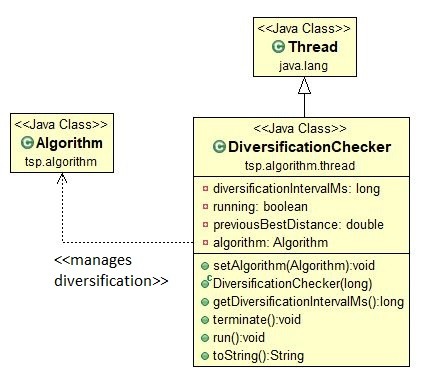
\includegraphics[height=8cm]{ClassDiversificationChecker.JPG}
\caption{Deklaracja klasy DiversificationChecker}
\end{figure}


\subsection{Zbieranie wyników}

Do zbierania danych został utworzony wątek, który co ustalony interwał (domyślnie- sekunda) sprawdza aktualne najlepsze znalezione rozwiązanie przez Algorytm, a następnie zapisuje je do pliku oraz, jeśli ustawiono, dodaje punkt na wyświetlanym wykresie.

\begin{figure}[H]
\centering
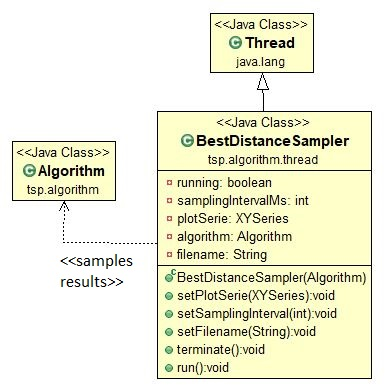
\includegraphics[height=8cm]{ClassBestDistanceSampler.JPG}
\caption{Deklaracja klasy BestDistanceSampler}
\end{figure}

\subsection{Lista Tabu}

Został zdefiniowany interfejs definiujący operacje, które można wynonać na liście tabu, a więc, dodanie ruchu oraz sprawdzenie czy dany ruch jest tabu. Taka struktura pozwala na dynamiczną podmianę używanej implementacji listy zakazów. W ramach projektu zdefiniowano dwie implementacje:
\begin{itemize}
\item TabuListDisabled - implementacja, która przy dodaniu ruchu do listy nie robi nic, a sprawdzenie czy ruch jest tabu zawsze zwraca odpowiedź "fałsz". Ta implementacja została zdefiniowana w celu umożliwienia wyłączenia listy tabu - algorytm staje się tradycyjnym przeszukiwaniem lokalnym.
\item TabuListImpl  - kolejka o ograniczonej wielkości
\end{itemize}

\begin{figure}[H]
\centering
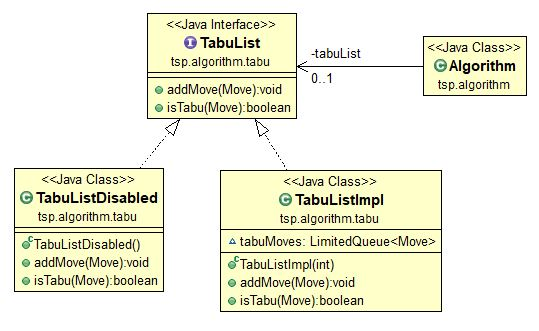
\includegraphics[height=7.5cm]{TabuList.JPG}
\caption{Interfejs Tabu List oraz jego implementacje}
\end{figure}


\subsection{Ruchy}

W projekcie zostały zdefiniowane trzy rodzaje ruchów (zmian aktualnego rozwiązania). Zostaną one opisane w kolejnych podpunktach.

\begin{figure}[H]
\centering
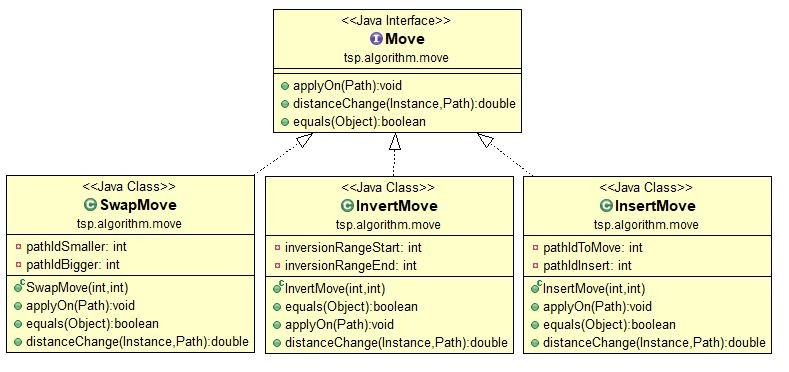
\includegraphics[width=17cm]{Move.JPG}
\caption{Interfejs Move oraz jego implementacje}
\end{figure}

\subsubsection{SwapMove}
Ruch polega na zamianie miejscami dwóch miast  w ścieżce (zadanych jako ich pozycje).\\[0.3cm]
Parametry: 
\begin{itemize}
\item pathIdSmaller - id pierwszego z elementów ścieżki do wymiany (mniejsze)
\item pathIdBigger - id drugiego z elementów ścieżki do wymiany (większe)
\end{itemize}
Dziedzina: 
\begin{itemize}
\item pathIdSmaller > 0, pathIdSmaller < path.size() - 2
\item pathIdBigger > pathIdSmaller, pathIdBigger < path.size() - 1

\end{itemize}
Przykład:

\begin{figure}[H]
\centering
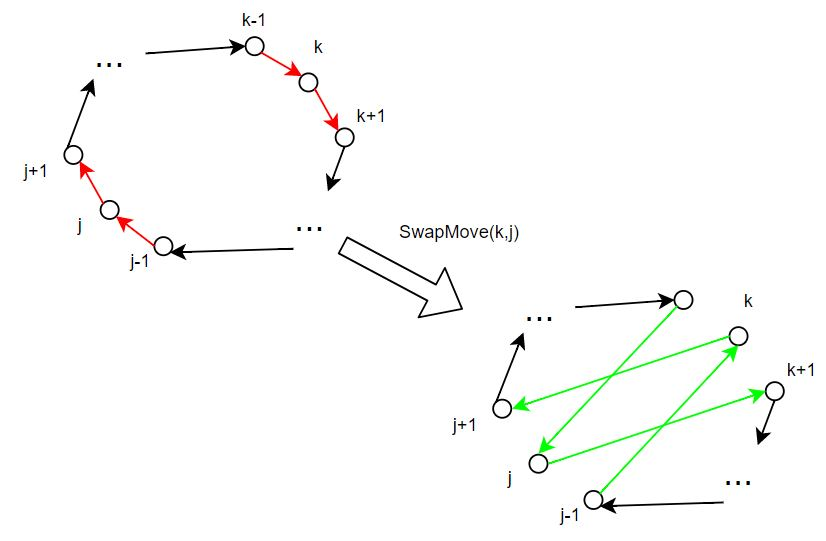
\includegraphics[height=10cm]{SwapMove.JPG}
\caption{Przykład ruchu SwapMove (źródło własne)}
\end{figure}

\newpage
\subsubsection{InsertMove}
Ruch polega na wstawieniu miasta będącego na zadanej pozycji w inną zadaną pozycję w ścieżce.\\[0.3cm]
Parametry: 
\begin{itemize}
\item pathIdToMove - id elementu ścieżki do przeniesienia
\item pathIdInsert - id elementu ścieżki, w które ma zostać wstawiony element przenoszony
\end{itemize}
Dziedzina: 
\begin{itemize}
\item pathIdToMove > 0, pathIdInsert > 0, pathIdToMove != pathIdInsert

\end{itemize}
Przykład:

\begin{figure}[H]
\centering
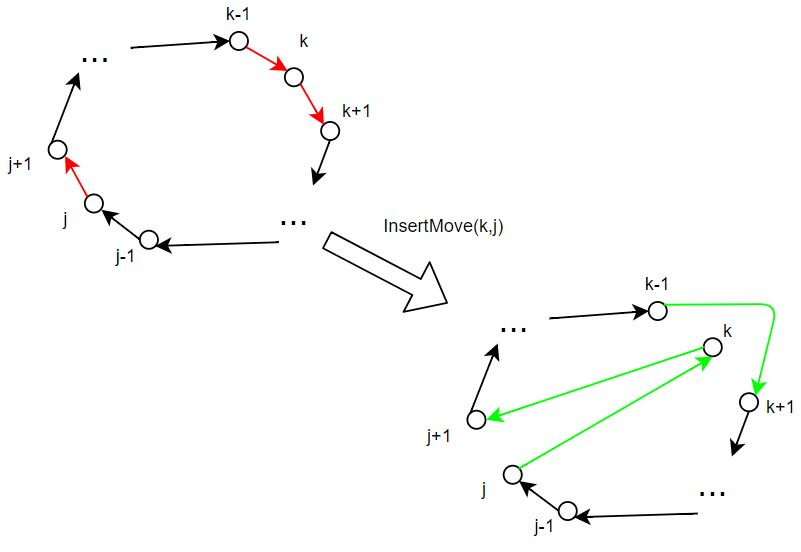
\includegraphics[height=10cm]{InsertMove.JPG}
\caption{Przykład ruchu InsertMove (źródło własne)}
\end{figure}
\newpage

\subsubsection{InvertMove}
Ruch polega na odwróceniu kolejności w podścieżce (sekwencja miast) zawartej w ścieżce.\\[0.3cm]
Parametry: 
\begin{itemize}
\item inversionRangeStart - id elementu będącego początkiem podścieżki
\item inversionRangeEnd - id elementu będącego końcem podścieżki
\end{itemize}
Dziedzina: 
\begin{itemize}
\item inversionRangeStart > 0, inversionRangeStart < path.size() - 2
\item inversionRangeEnd > inversionRangeStart, inversionRangeEnd < path.size() - 1

\end{itemize}
Przykład:

\begin{figure}[H]
\centering
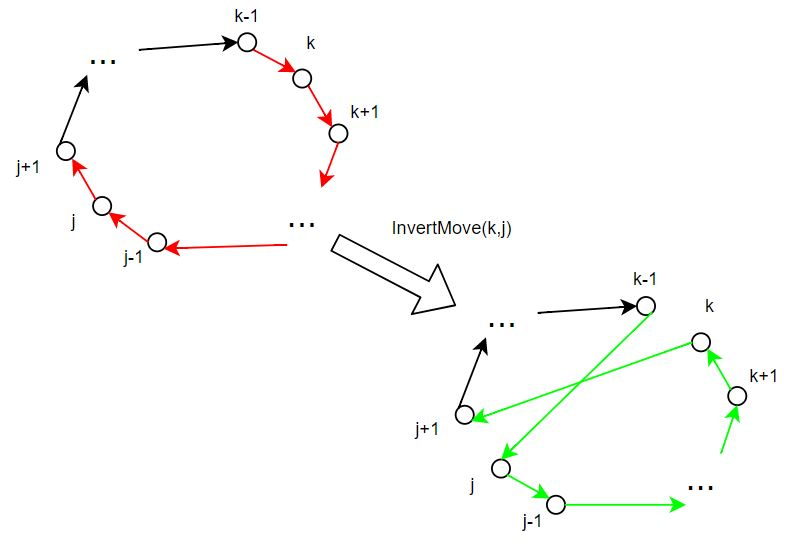
\includegraphics[height=10cm]{InvertMove.JPG}
\caption{Przykład ruchu InvertMove (źródło własne)}
\end{figure}

\newpage
\subsection{Generatory sąsiedztwa}

Dla każdego z wyżej opisanych ruchów został utworzony generator sąsiedztwa, który zajmuje się generowaniem listy możliwych ruchów dla danej ścieżki (z uwzględnieniem dziedziny konkretnego ruchu).

\begin{figure}[H]
\centering
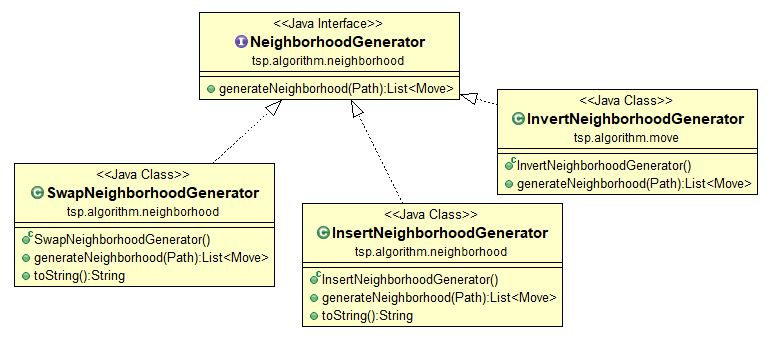
\includegraphics[width=17cm]{ClassNeighborhoodGenerator.JPG}
\caption{Interfejs NeighborhoodGenerator oraz jego implementacje}
\end{figure}

\subsection{Algorytm}
\subsubsection{Zależności}
Zależności algorytmu (wyżej opisane klasy) muszą zostać ustawione przy konstrukcji instancji klasy Algorithm. 
\subsubsection{Działanie}
W pierwszej kolejności algorytm uruchamia wątki, do których referencje zostały ustawione przy jego konkstrukcji. Uruchamiany jest wątek typu AlgorithmTerminator, który zatrzyma algorytm po ustalonym czasie, wątek BestDistanceSampler służący do próbkowania wyników oraz, jeśli ustawiono, wątek zarządzający dywersyfikacją.
\\[0.3cm]Następnie zostaje wygenerowane rozwiązanie za pomocą metody zachłannej. W sąsiedztwie tak otrzymanego rozwiązania poszukiwane są co raz to lepsze rozwiązania. Za pomocą generatora możliwych ruchów w kazdej iteracji generowane są wszystkie możliwe ruchy, a następnie spośród tych, które nie są w danym momencie zakazane, wybiera się rozwiązanie które najlepiej wpłynie na wynik. Ruch, który został wykonany w celu uzyskania danego rozwiązania staje się ruchem zakazanym. 
\\[0.3cm]W przypadku wykrycia flagi dywersyfikacji, generowane jest losowe rozwiązanie. W przypadku zakończenia pracy przez wątek AlgorithmTerminator, najlepszy uzyskany do tej pory wynik jest zwracany.

\begin{figure}[H]
\centering
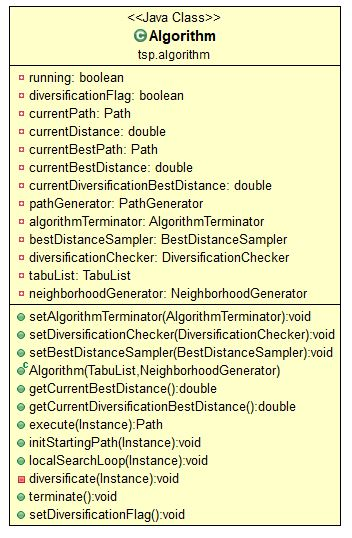
\includegraphics[width=8cm]{ClassAlgorithm.JPG}
\caption{Metody i atrybuty klasy Algorithm}
\end{figure}

\section{Wyniki badań}

Po zaimplementowaniu algorytmu oraz klas pomoczniczych zostały przeprowadzone testy jakościowe. Testy zostały przeprowadzone na trzech instancjach o różnej wielkości. Dla każdej z instancji zbadano wyniki otrzymane w przeciągu 6 minut dla różnych rodzajów sąsiedztwa, z zastosowaniem dywersyfikacji oraz bez. 

\subsection{Parametry}

\begin{itemize}
\item Kadencja listy zakazów została ustawiona na trzykrotność wielkości problemu (3*N).
\item Ograniczenie czasowe algorytmu zostało ustawione na 6 minut.
\item Interwał sprwadzenia dywersyfikacji został ustawiony na 30 sekund.
\end{itemize}

\newpage
\subsection{Instancja - eil101.tsp}

Optymalna długość ścieżki: 629

\subsubsection{Tabela zbiorcza}

\begin{figure}[H]
\centering
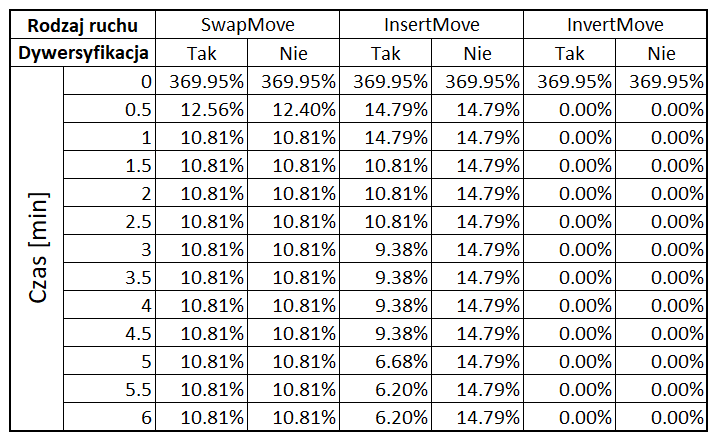
\includegraphics[height=9cm]{101.PNG}
\caption{Tabela zbiorcza dla instancji eil101.tsp}
\end{figure}


\subsubsection{Swap Move}

\begin{figure}[H]
\centering
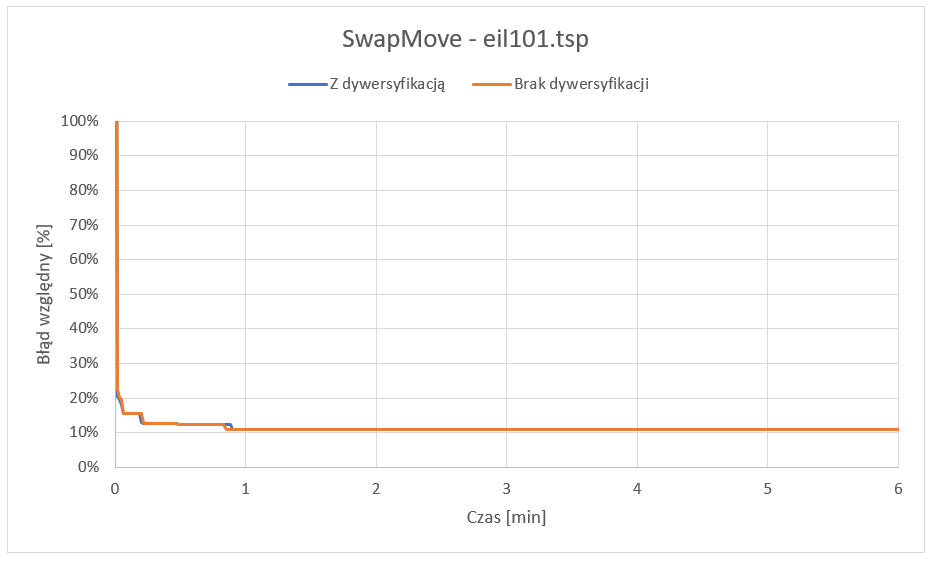
\includegraphics[height=10cm]{SwapMove101.PNG}
\caption{Zależnośc błędu względnego od czasu dla SwapMove (eil101.tsp)}
\end{figure}

\subsubsection{Insert Move}

\begin{figure}[H]
\centering
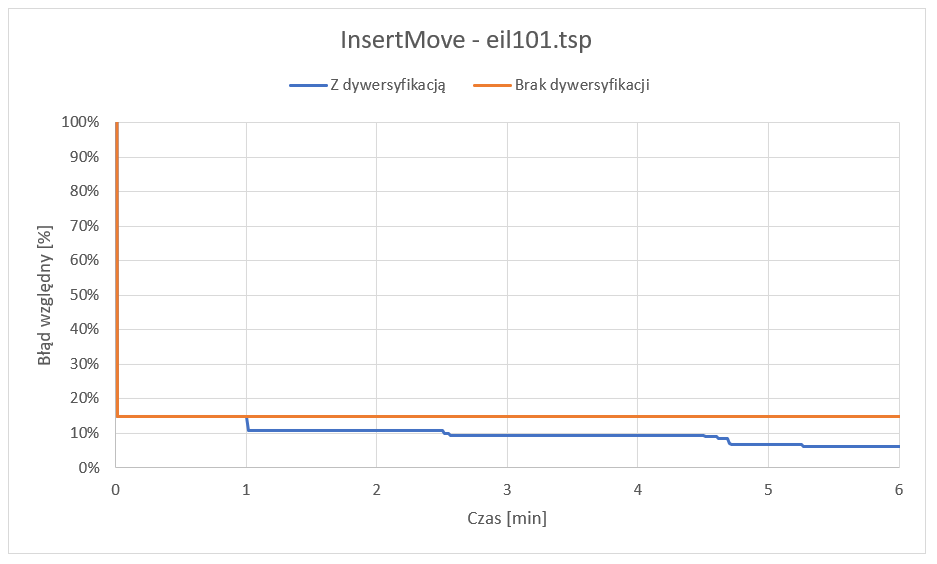
\includegraphics[height=10cm]{InsertMove101.PNG}
\caption{Zależnośc błędu względnego od czasu dla InsertMove (eil101.tsp)}
\end{figure}

\subsubsection{Invert Move}
\begin{figure}[H]
\centering
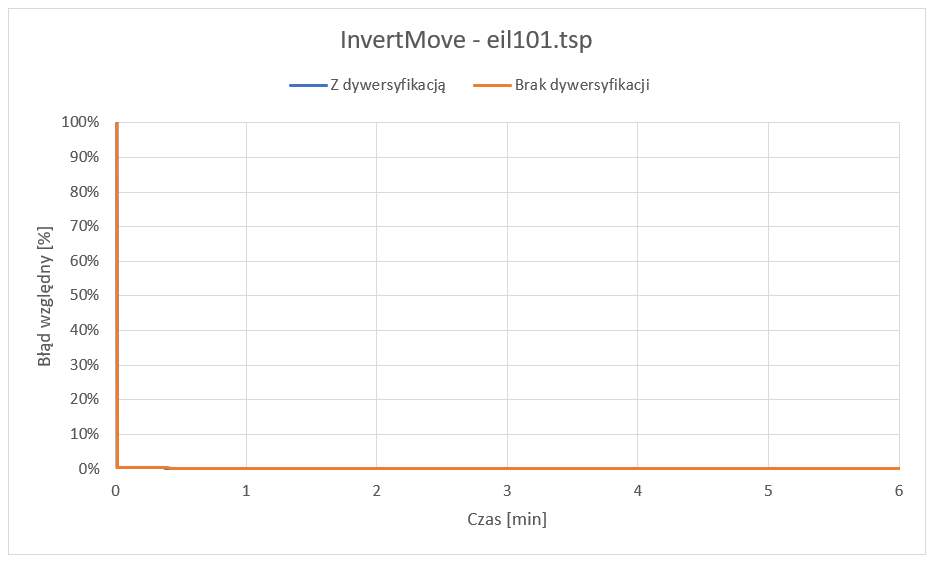
\includegraphics[height=10cm]{InvertMove101.PNG}
\caption{Zależnośc błędu względnego od czasu dla InvertMove (eil101.tsp)}
\end{figure}

\subsection{Instancja - rbg403.atsp}

Optymalna długość ścieżki: 629

\subsubsection{Tabela zbiorcza}

\begin{figure}[H]
\centering
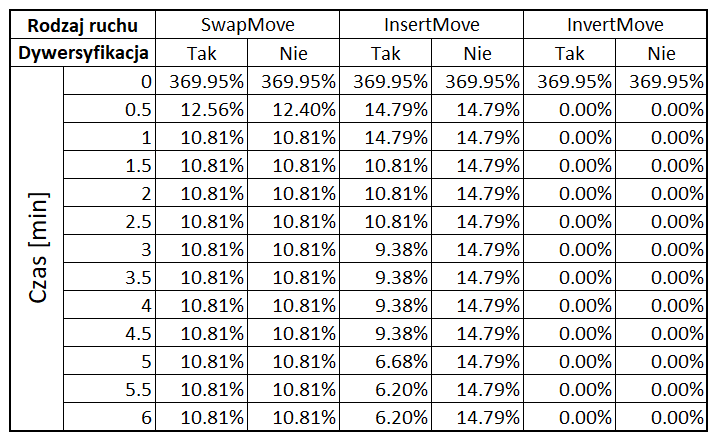
\includegraphics[height=9cm]{101.PNG}
\caption{Tabela zbiorcza dla instancji rbg403.atsp}
\end{figure}


\subsubsection{Swap Move}

\begin{figure}[H]
\centering
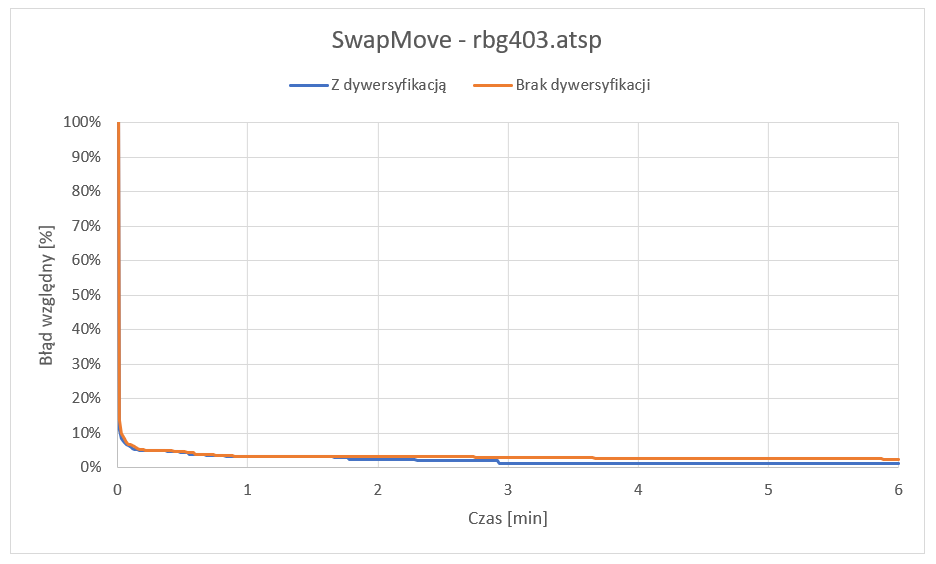
\includegraphics[height=10cm]{SwapMove403.PNG}
\caption{Zależnośc błędu względnego od czasu dla SwapMove (rbg403.atsp)}
\end{figure}

\subsubsection{Insert Move}

\begin{figure}[H]
\centering
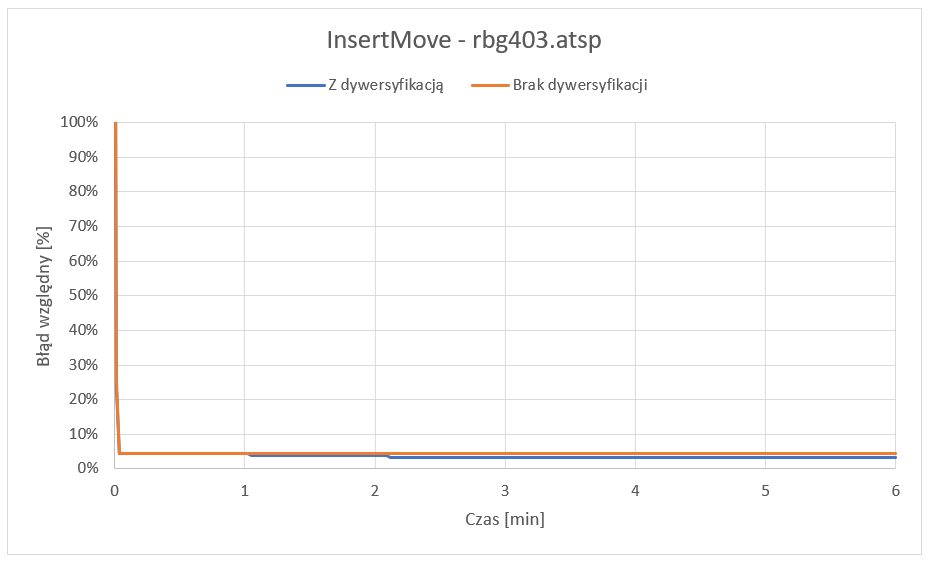
\includegraphics[height=10cm]{InsertMove403.PNG}
\caption{Zależnośc błędu względnego od czasu dla InsertMove (rbg403.atsp)}
\end{figure}

\subsubsection{Invert Move}
\begin{figure}[H]
\centering
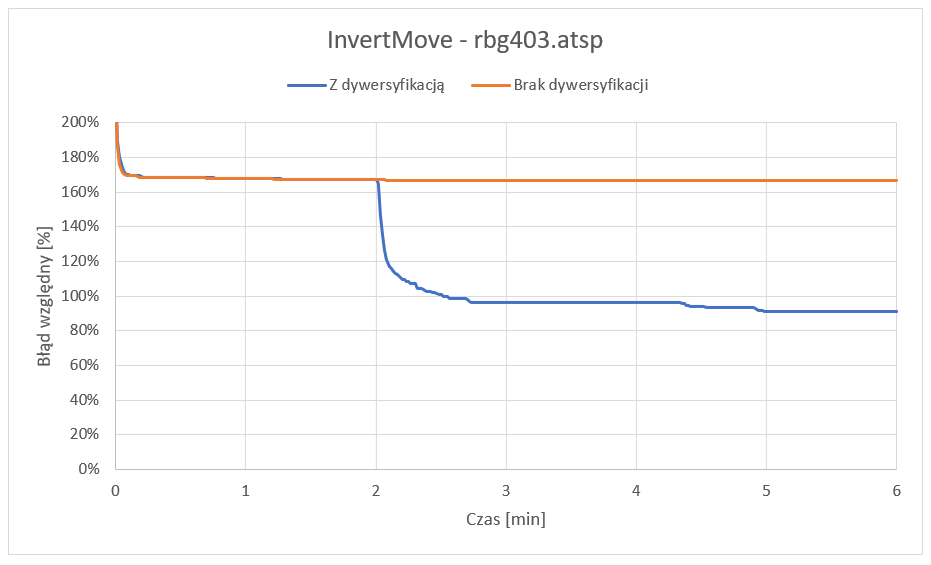
\includegraphics[height=10cm]{InvertMove403.PNG}
\caption{Zależnośc błędu względnego od czasu dla InvertMove (rbg403.atsp)}
\end{figure}

\subsection{Instancja - d1291.tsp}

Optymalna długość ścieżki: 50801

\subsubsection{Tabela zbiorcza}

\begin{figure}[H]
\centering
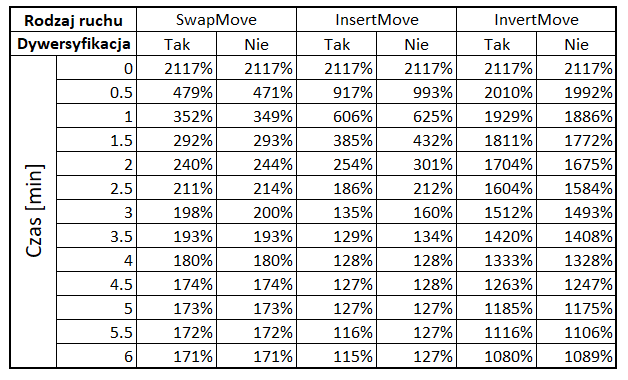
\includegraphics[height=9cm]{1291.PNG}
\caption{Tabela zbiorcza dla instancji d1291.tsp}
\end{figure}


\subsubsection{Swap Move}

\begin{figure}[H]
\centering
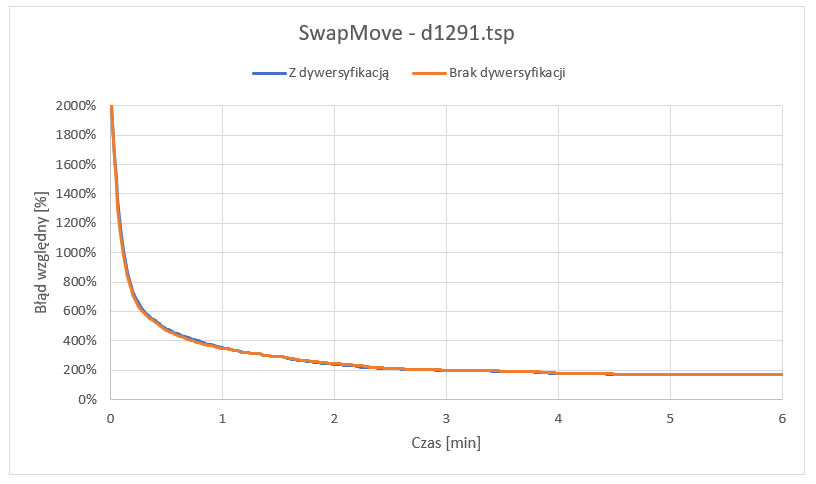
\includegraphics[height=10cm]{SwapMove1291.PNG}
\caption{Zależnośc błędu względnego od czasu dla SwapMove (d1291.tsp)}
\end{figure}

\subsubsection{Insert Move}

\begin{figure}[H]
\centering
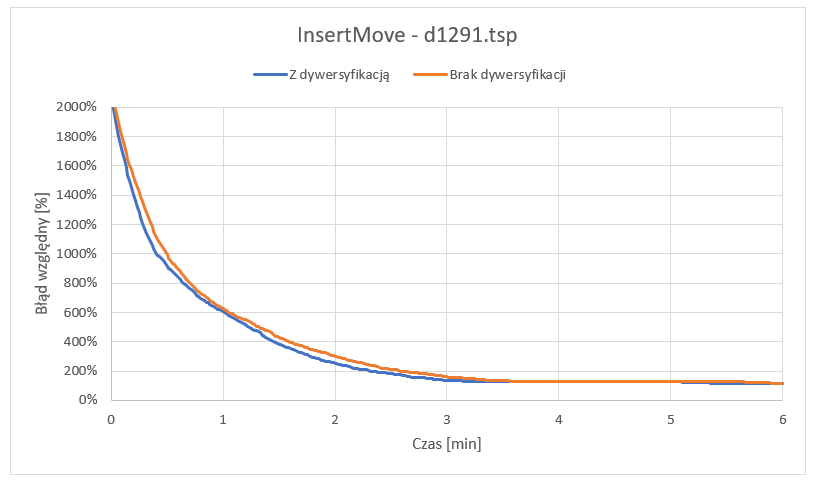
\includegraphics[height=10cm]{InsertMove1291.PNG}
\caption{Zależnośc błędu względnego od czasu dla InsertMove (d1291.tsp)}
\end{figure}

\subsubsection{Invert Move}
\begin{figure}[H]
\centering
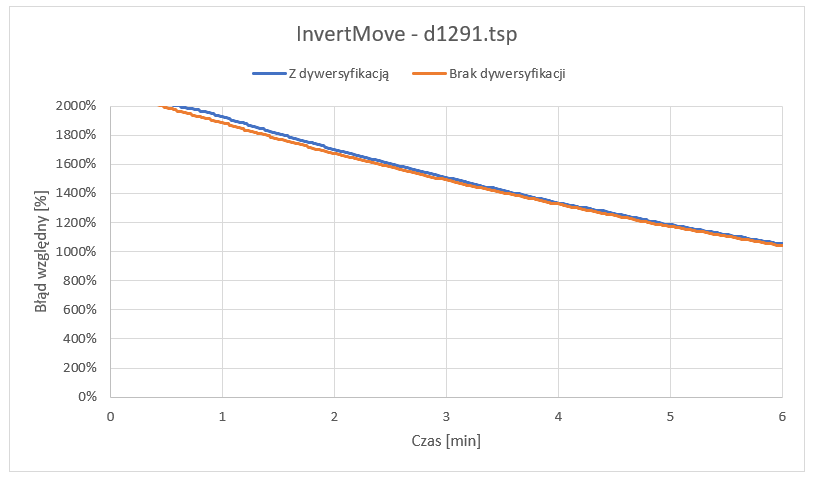
\includegraphics[height=10cm]{InvertMove1291.PNG}
\caption{Zależnośc błędu względnego od czasu dla InvertMove (d1291.tsp)}
\end{figure}

\section{Podsumowanie, wnioski}

Zaimplementowany algorytm oparty na metodyce przeszukiwania z zakazami skutecznie radził sobie z znajdywaniem rozwiązań bliskich optymalnemu w krótkim czasie, mimo dużych rozmiarów instancji. 
\begin{itemize}
\item Dla instancji eil101.tsp oraz sąsiedztwa InvertMove udało się znaleźć rozwiązanie, które zostało uznane za optymalne na podstawie danych zamieszczonych na stronie TSPLIB95.
\item Dla instancji o większym rozmiarze sąsiedztwo InvertMove okazało się być najmniej skuteczne. Być może jakość rozwiązań zwiększyłoby ustawienie mniejszej wartości kadencji.
\item Dla instancji o rozmiarze 1291 wyniki z użyciem dywersyfikacji nie różnią się znacząco od wyników bez jej użycia. Wynika to z krótkiego czasu badania, podczas którego nie udało się osiągnąć minimum lokalnego, z którego algorytm nie byłby stanie wyjść.
\item Dla pozostałych przypadków mechanizm dywersyfikacji pozytywnie wpłynął na jakość wyników. Znaczną poprawę wyniku przy zastosowaniu dywersyfikacji widać na Rysunku 21.
\item Nie można jednoznacznie określić, które sąsiedztwo jest najlepsze. Skuteczność sąsiedztwa zależy od konkretnego problemu. W celu uzyskania najlepszych wyników powinno się dobrać sąsiedztwo oraz kadencję listy zakazów, np. doświadczalnie. Sąsiedztwa można również wymieszać ze sobą, jak również jego wybór pozostawić jako element losowy w iteracji algorytmu.
\item Metody aproksymacyjne pozwalają na otrzymywanie (często) zadowalających wynikow nawet dla dużych instancji problemu.
\end{itemize}




















\end{document}